\documentclass{simple}

\title[vmchecker]{Administrarea prin interfață web a vmchecker}
\institute{ROSEdu Summer of Code}
\author[Răzvan Deaconescu]{Cosmin Didii \& \textbf{Răzvan Deaconescu} \\
cosmin.didii@gmail.com \& razvan@rosedu.org}
\date{7 octombrie 2012}

\begin{document}

\frame{\titlepage}

\begin{frame}{vmchecker}
  \begin{itemize}
    \item soluție pentru evaluarea automată a temelor de casă
    \item folosită la o serie de materii din facultate
    \item utilizare în creștere
    \item dezvoltată la RSoC v2 (2008)
    \item folosită din 2008-2009
    \item suport inițial de VMware
    \item adăugat suport, la diplomă 2012, pentru VirtualBox, LXC și KVM
  \end{itemize}
\end{frame}

\begin{frame}{Arhitectura vmchecker}
  \begin{figure}
    \centering
    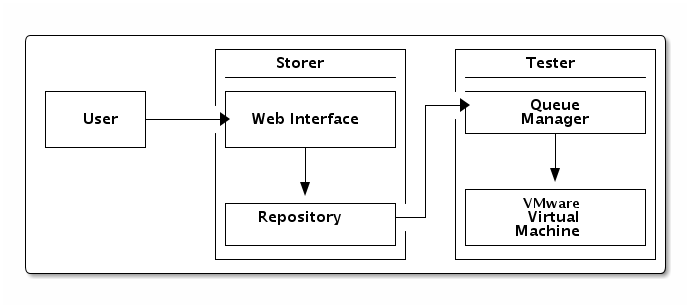
\includegraphics[width=0.8\textwidth]{img/vmchecker-architecture} \\
    \tiny{Lucrare de diplomă Vali Goșu}
  \end{figure}
\end{frame}

\begin{frame}{Interfața cu utilizatorul}
  \begin{itemize}
    \item WebUI pentru studenți
      \begin{itemize}
        \item upload teme
        \item selectare discipline și teme
        \item vizualizare rezultate
        \item scrisă în GWT (\textit{Google Web Toolkit)}
      \end{itemize}
    \item CLI pentru cadre didactice
      \begin{itemize}
        \item accesare fișiere cod sursă
        \item vizualizare fișiere cod sursă
        \item resubmitere teme
        \item actualizare bază de date
        \item evaluare teme
      \end{itemize}
    \item CLI pentru administratori
  \end{itemize}
\end{frame}

\begin{frame}{Neajunsuri și propuneri de soluționare}
  \begin{itemize}
    \item interfață neatractivă pentru cadre didactice -- interfață Web
    \item configurarea dificilă și descentralizată pentru admin -- interfață
      Web
    \item absența unui dezvoltator de interfață web cu permanență în
      facultate (Claudiu Gheorghe nu mai poate aloca tim) -- atragerea unui
      dezvoltator pe termen lung
    \item proiect nedocumentat -- documentarea acestuia în paralel cu
      dezvoltarea
    \item titlu necorespunzător al proiectului -- pe parcurs am adăugat
      cerința de adăugare de WebUI și pentru client (pentru unificare)
  \end{itemize}
\end{frame}

\begin{frame}{Tehnologii}
  \begin{itemize}
    \item Git \& GitHub
    \item PHP, CSS, JS, HTML
    \item folosirea informațiilor din interfața veche
  \end{itemize}
\end{frame}

\begin{frame}{Pași urmați}
  \begin{itemize}
    \item o abordare mai degrabă reactivă
    \item kicking-off: conturi GitHub, elf.cs.pub.ro
    \item scrie cod, funcționalități de bază
    \item feedback pe funcționalități, trecerea la design
    \item user stories pe trei roluri: student, teacher, admin (GitHub wiki)
    \item (re)implementare de funcționalități în conformitate cu user stories
    \item feedback pe intefață/funcționalitate
  \end{itemize}
\end{frame}

\begin{frame}{Comunicare/colaborare}
  \begin{itemize}
    \item Skype și e-mail (e-mail a fost baza)
    \item sesiuni de feedback
    \item sesiunile de raportare erau incluse în blog posts
    \item focus pe ,,calitate'' nu ,,cantitate''
    \item resimțită lipsa unei comunități în cadrul proiectului (doar discuții
      unu la unu)
  \end{itemize}
\end{frame}

\begin{frame}{Demo}
  \begin{itemize}
    \item old interface (WebUI/CLI)
    \item new interface (WebUI)
    \item repo browse
  \end{itemize}
\end{frame}

\begin{frame}{Concluzie}
  \begin{itemize}
    \item interfață actualizată în PHP
    \item facilități complete pentru studenți, cadre didactice, administratori
    \item dezvoltator de interfață, integrare în vmchecker planificată
    \item skill-uri de software development
  \end{itemize}
\end{frame}

\begin{frame}{Further Work}
  \begin{itemize}
    \item mod de publicare automată a codului pentru WebUI (post-receive hook)
    \item definitivarea interfeței
    \item dezvoltarea de teste unitare
    \item test, test and test; and then test; and get feedback
    \item integrarea în vmchecker (semestrul 2 2012-2013)
    \item integrare facilități de feedback direct în interfață
    \item unificat repository-uri, pagină de Facebook etc.
    \item promovat vmchecker în alte materii din facultate
    \item pachet de instalare vmchecker
  \end{itemize}
\end{frame}

\begin{frame}{Post Performance Analysis}
  \begin{itemize}
    \item absența unor discuții legate de partea de software engineering și
      specificații de proiect pe componente
    \item design first, implement later (business layer vs. application layer)
    \item e utilă dezvoltarea \textbf{în} cadrul unui cod deja existent și a
      unei comunități existente
    \item folosire precară a Git
    \item tehnici de dezvoltare Web
    \item aspecte de utilizabilitate
    \item consecvența denumirilor și a interfeței
  \end{itemize}
\end{frame}

\begin{frame}{Metrici}
  \begin{itemize}
    \item 2992 linii în fișiere .php
    \item 878 linii în fișiere .css
    \item 458 linii în fișiere .js
    \item pagină de User Stories pe wiki
  \end{itemize}
\end{frame}

\begin{frame}{Resurse utile}
  \begin{itemize}
    \item \url{https://github.com/cosmin1123/vmchecker}
    \item \url{https://elf.cs.pub.ro/vmchecker-rsoc/login.php}
    \item \url{https://github.com/vmchecker/vmchecker}
    \item \url{https://elf.cs.pub.ro/vmchecker/ui/}
    \item \url{http://lists.rosedu.org/listinfo/vmchecker-dev}
    \item \texttt{vmchecker-request@cursuri.cs.pub.ro}
  \end{itemize}
\end{frame}

\end{document}
